Basierend auf den Anforderungsdefinitionen, stellt die Implementierung die Umsetzung des beschriebenen Entwurfs innerhalb des Prozessablaufs dar. 

Um ein besseres Verständnis zu erlangen, wird das Ayoy-Plugin im Rahmen der Implementierung verschiedenen Tests unterworfen, die jeweils einen erwartenden Zustand aufweisen und basierend auf den SOLL-Prozess die jeweilige Reaktion des Entwicklers beschreiben.

An dieser Stelle erfolgt das Testen des Ayoy-Plugins mittels eines einfachen Maven-Programms, welches aussschließlich einen String mit 'Hello World' ausgibt.

Um das Plugin automatisiert innerhalb dieses Programmes einzubinden, wurde der entsprechende Aufruf innerhalb der pom.xml eingebettet. 

Obwohl das Programm ein einfaches Beispiel darstellt, werden die Stärken und die Schwachstellen des Ayoy-Plugins verdeutlicht und erleichtert eine mögliche Fehlersuche. 

\paragraph{Fall 1: Keine Auffälligkeiten innerhalb der Lizenzen}$~$

Dieser Fall beschreibt die Prüfung, bei der alle Lizenzen und deren Abhängigkeiten kein Copyleft aufweisen und daher innerhalb des Projektes verwendet und an die Stakeholder ausgeliefert werden können. 

Innerhalb des Programmes wurden Lizenzen mit starker Copyleft aus der pom.xml entfernt, fehlende Lizenzen innerhalb der licence.xml hinzugefügt und Abhängigkeiten, die aussschließlich zu Testzwecken verwendet wurden, innerhalb der allowedMissingLicence.xml eingebettet.  

\begin{itemize}
    \item \textbf{Situation}: Alle Lizenzen und deren Abhängigkeiten sind \textit{erlaubt}
    
    \begin{figure}[h]
        \centering
        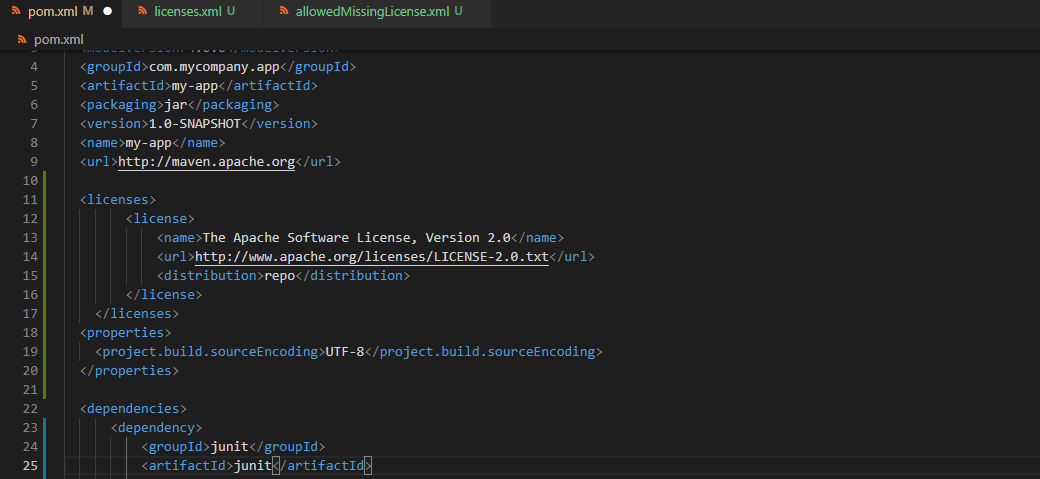
\includegraphics[scale=0.5]{Bilder/Fall1Situation.png}
    \end{figure}

    \item \textbf{Erwarteter Zustand}: Build-Prozess wird \textit{erfolgreich} durchgeführt 
    
    \begin{figure}[h]
        \centering
        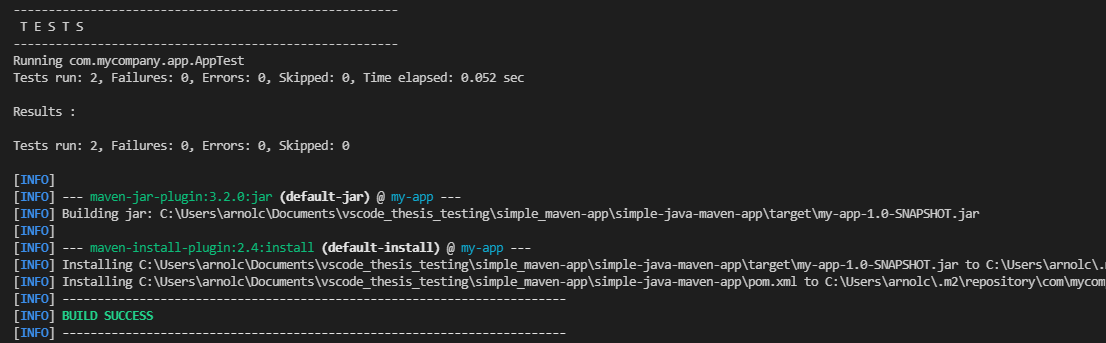
\includegraphics[scale=0.5]{Bilder/Fall1Zustand.png}
    \end{figure}

    \item \textbf{Reaktion anhand des Soll-Prozesses}: Entwickler kann innerhalb des Softwareentwicklungsprozesses weiter verfahren. 
\end{itemize}

\paragraph{Fall 2: Verwendung von Lizenzen mit starker Copyleft} $~$

Dieser Fall beschreibt die Prüfung, bei der Lizenzen erkannt wurden, die ein starkes Copyleft aufweisen und daher nicht in den Softwareentwicklungsprozesses eingebunden werden sollten.

Innerhalb des Programmes wurde beabsichtigt die GNU, also ein Lizenzmodell mit starker Copyleft der pom.xml hinzugefügt, fehlende Lizenzen innerhalb der licence.xml hinzugefügt und Abhängigkeiten, die aussschließlich zu Testzwecken verwendet wurden, innerhalb der allowedMissingLicence.xml eingebettet. 

\begin{itemize}
    \item \textbf{Situation}: Einige verwendete Lizenzen weisen \textit{unerlaubte} Lizenmodelle auf
    
    \begin{figure}[h]
        \centering
        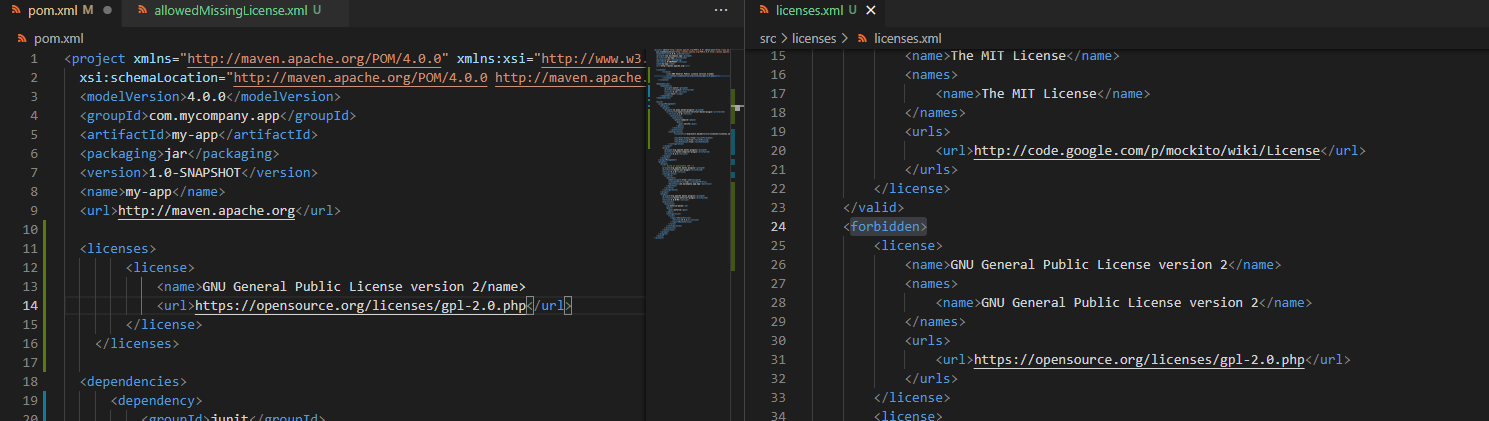
\includegraphics[scale=0.4]{Bilder/Fall2Situation.png}
    \end{figure}

    \item \textbf{Erwarteter Zustand}: Build-Prozess schlägt \textit{fehl} 
    
    \begin{figure}[h]
        \centering
        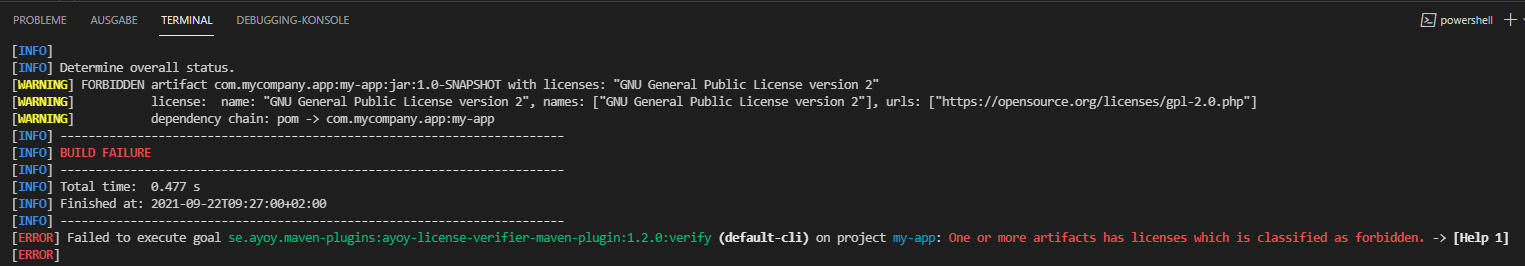
\includegraphics[scale=0.4]{Bilder/Fall2Zustand.png}
    \end{figure}

    \item \textbf{Reaktion anhand des Soll-Prozesses}: Entwickler muss die OSS-Thematik umgehend klären, indem entschieden wird, ob die Komponente entfernt wird oder der Copyleft-Effekt aufgrund einer Versionsänderung zustande kam. Kann die Komponente nicht ausgetauscht aber dringend benötigt werden, muss der Projektleiter entsprechend informiert werden.  
\end{itemize}

\paragraph{Fall 3: Verwendung von unbekannten Lizenzen} $~$

Dieser Fall beschreibt die Prüfung, bei der Lizenzen innerhalb der pom.xml erkannt wurden, die bisher nicht in der licence.xml vorhanden sind und daher für das Plugin als unbekannt gelten. 

Innerhalb des Programmes wurden unbekannte Lizenzen der pom.xml hinzugefügt, die innerhalb der licence.xml noch nicht vorhanden sind und Abhängigkeiten, die aussschließlich zu Testzwecken verwendet wurden, innerhalb der allowedMissingLicence.xml eingebettet. 

\begin{itemize}
    \item \textbf{Situation}: Einige verwendete Lizenzen weisen \textit{unbekannte} Lizenmodelle auf
    
    \begin{figure}[h]
        \centering
        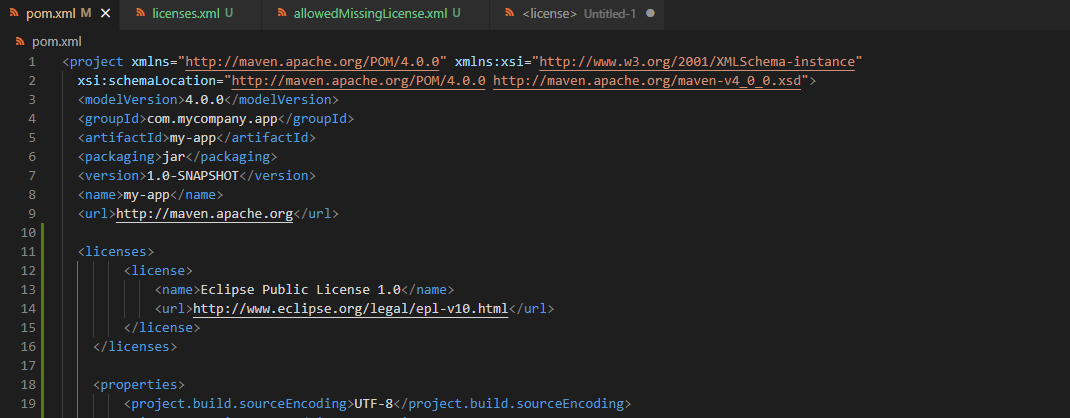
\includegraphics[scale=0.5]{Bilder/Fall3Situation.png}
    \end{figure}

    \item \textbf{Erwarteter Zustand}: Build-Prozess schlägt \textit{fehl} 
    
    \begin{figure}[h]
        \centering
        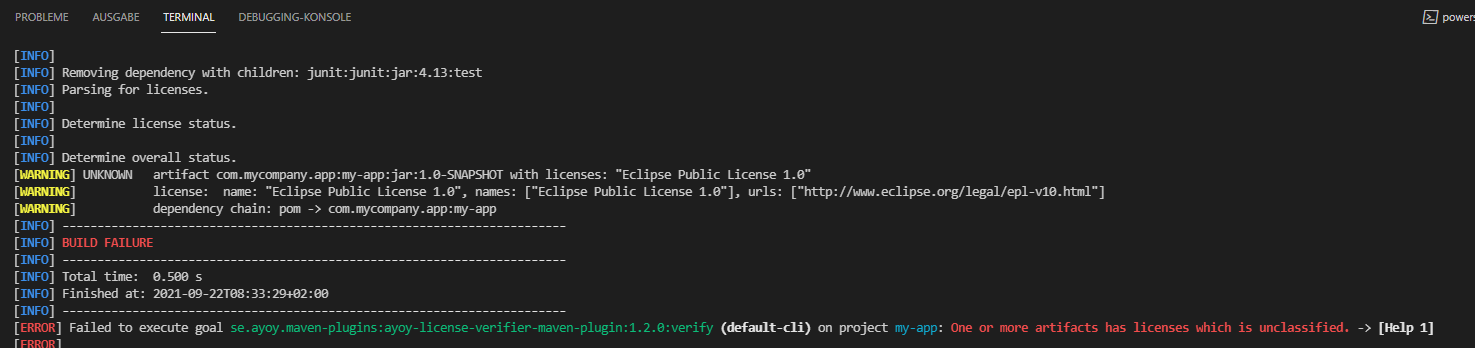
\includegraphics[scale=0.4]{Bilder/Fall3Zustand.png}
    \end{figure}

    \item \textbf{Reaktion anhand des Soll-Prozesses}: Entwickler muss zunächst anhand des Lizenzmodells, den Status des Copylefts recherchieren und anschließend die Lizenzen innerhalb der licence.xml an der entsprechenden Stelle hinzufügen. 
\end{itemize}

\paragraph{Fall 4: Verwendung von unbekannten Abhängigkeiten} $~$

Dieser Fall beschreibt die Prüfung, bei der Lizenzen innerhalb Abhängigkeiten erkannt wurden, die bisher nicht in der licence.xml vorhanden sind.

Im Rahmen dieses Falles werden zudem transitive Abhängigkeiten deutlich, also Abhängigkeiten die ihrerseits weitere Abhängigkeiten besitzen. 

Innerhalb des Programmes wurden unbekannte Abhängigkeiten der pom.xml hinzugefügt, dessen Lizenzen innerhalb der licence.xml noch nicht vorhanden sind und Abhängigkeiten, die aussschließlich zu Testzwecken verwendet wurden, nicht innerhalb der allowedMissingLicence.xml eingebettet. 

\begin{itemize}
    \item \textbf{Situation}: Einige verwendete Abhängigkeiten weisen \textit{unbekannte} Lizenmodelle auf
    
    \begin{figure}[h]
        \centering
        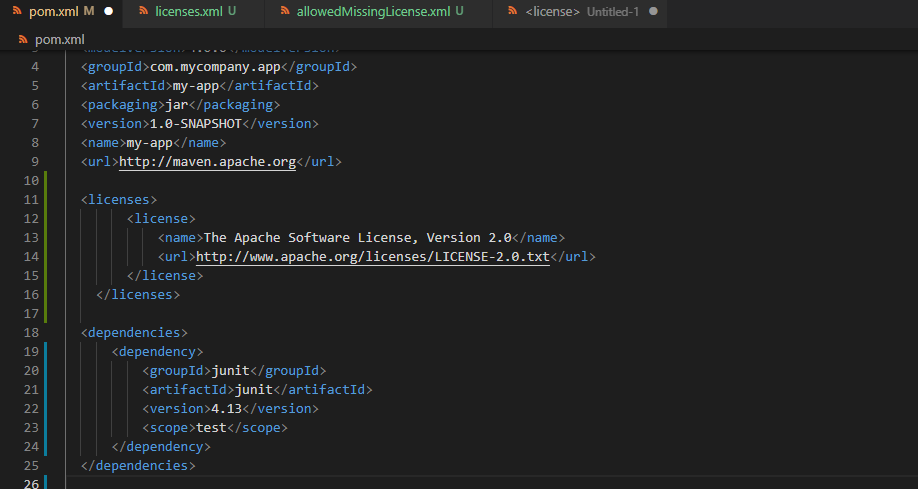
\includegraphics[scale=0.5]{Bilder/Fall4Situation.png}
    \end{figure}

    \item \textbf{Erwarteter Zustand}: Build-Prozess schlägt \textit{fehl} 
    
    \begin{figure}[h]
        \centering
        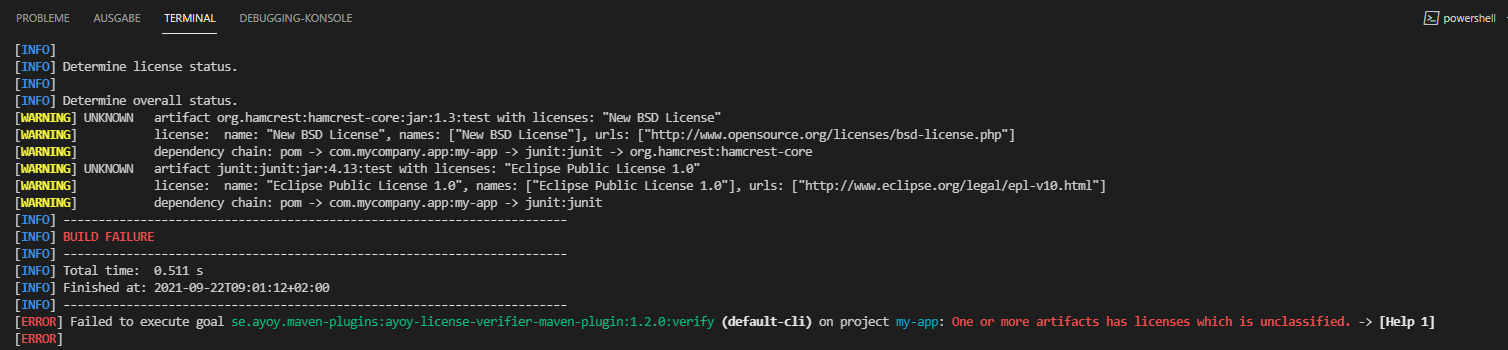
\includegraphics[scale=0.4]{Bilder/Fall4Zustand.png}
    \end{figure}

    \item \textbf{Reaktion anhand des Soll-Prozesses}: Entwickler muss zunächst anhand des Lizenzmodells der Abhängigkeit, den Status des Copylefts über mehrere Abhängigkeiten recherchieren und anschließend die Lizenzen innerhalb der licence.xml an der entsprechenden Stelle hinzufügen. Sollte es sich hierbei um ein Lizenzmodell handeln, welches aussschließlich zu Testzwecken verwendet wird, muss die Abhängigkeit der allowedMissingLicence.xml zusätzlich hinzugefügt werden. 
\end{itemize}

\paragraph{Fall 5: Verwendung von Abhängigkeiten zu Testzwecken} $~$

Dieser Fall beschreibt die Prüfung, bei der Abhängigkeiten erkannt wurden, die ihrerseits ein Lizenzmodell mit starker Copyleft aufweisen und aussschließlich für Testzwecke verwendet werden. 

Innerhalb des Programmes wurden Abhängigkeiten der pom.xml hinzugefügt, dessen Lizenzen innerhalb der licence.xml unter 'forbidden' stehen und nicht innerhalb der allowedMissingLicence.xml eingebettet sind. 

\begin{itemize}
    \item \textbf{Situation}: Einige verwendete Abhängigkeiten weisen \textit{unerlaubte} Lizenmodelle auf, die zum testen verwendet werden
    
    \begin{figure}[h]
        \centering
        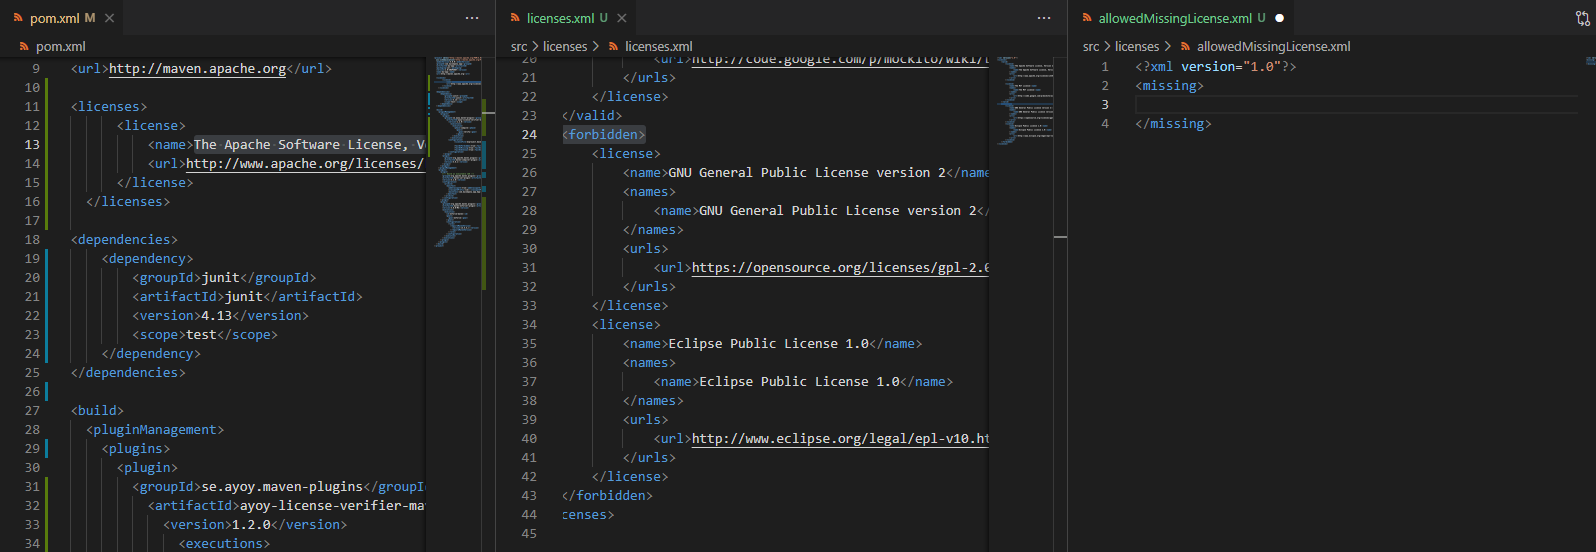
\includegraphics[scale=0.4]{Bilder/Fall5Situation.png}
    \end{figure}

    \item \textbf{Erwarteter Zustand}: Build-Prozess schlägt \textit{fehl} 

    \begin{figure}[h]
        \centering
        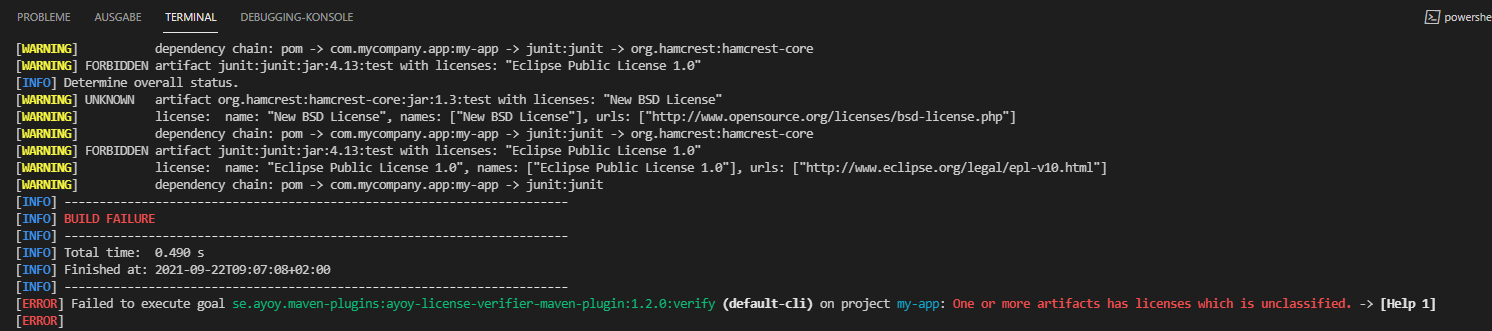
\includegraphics[scale=0.4]{Bilder/Fall5Zustand.png}
    \end{figure}

    \item \textbf{Reaktion anhand des Soll-Prozesses}: Entwickler muss zunächst sicherstellen, dass die verwendete Abhängigkeit aussschließlich für Testzwecke verwendet wird und dieses der allowedMissingLicence.xml hinzufügen. 
\end{itemize}
